%%%%%%%%%%%%%%%%%%%%%%%%%%%%%%%%%%%%%%%%%%%%%%%%%%%%%%%%%%%%%%%%%%%%%%%%%%%%%%%%
%Tutorial slides on Python.
%
% Author: FOSSEE 
% Copyright (c) 2009, FOSSEE, IIT Bombay
%%%%%%%%%%%%%%%%%%%%%%%%%%%%%%%%%%%%%%%%%%%%%%%%%%%%%%%%%%%%%%%%%%%%%%%%%%%%%%%%

\documentclass[14pt,compress]{beamer}
%\documentclass[draft]{beamer}
%\documentclass[compress,handout]{beamer}
%\usepackage{pgfpages} 
%\pgfpagesuselayout{2 on 1}[a4paper,border shrink=5mm]

% Modified from: generic-ornate-15min-45min.de.tex
\mode<presentation>
{
  \usetheme{Warsaw}
  \useoutertheme{infolines}
  \setbeamercovered{transparent}
}

\usepackage[english]{babel}
\usepackage[latin1]{inputenc}
%\usepackage{times}
\usepackage[T1]{fontenc}
\usepackage{amsmath}

% Taken from Fernando's slides.
\usepackage{ae,aecompl}
\usepackage{mathpazo,courier,euler}
\usepackage[scaled=.95]{helvet}

\definecolor{darkgreen}{rgb}{0,0.5,0}

\usepackage{listings}
\lstset{language=Python,
    basicstyle=\ttfamily\bfseries,
    commentstyle=\color{red}\itshape,
  stringstyle=\color{darkgreen},
  showstringspaces=false,
  keywordstyle=\color{blue}\bfseries}

%%%%%%%%%%%%%%%%%%%%%%%%%%%%%%%%%%%%%%%%%%%%%%%%%%%%%%%%%%%%%%%%%%%%%%
% Macros
\setbeamercolor{emphbar}{bg=blue!20, fg=black}
\newcommand{\emphbar}[1]
{\begin{beamercolorbox}[rounded=true]{emphbar} 
      {#1}
 \end{beamercolorbox}
}
\newcounter{time}
\setcounter{time}{0}
\newcommand{\inctime}[1]{\addtocounter{time}{#1}{\tiny \thetime\ m}}

\newcommand{\typ}[1]{\lstinline{#1}}

\newcommand{\kwrd}[1]{ \texttt{\textbf{\color{blue}{#1}}}  }

%%% This is from Fernando's setup.
% \usepackage{color}
% \definecolor{orange}{cmyk}{0,0.4,0.8,0.2}
% % Use and configure listings package for nicely formatted code
% \usepackage{listings}
% \lstset{
%    language=Python,
%    basicstyle=\small\ttfamily,
%    commentstyle=\ttfamily\color{blue},
%    stringstyle=\ttfamily\color{orange},
%    showstringspaces=false,
%    breaklines=true,
%    postbreak = \space\dots
% }


%%%%%%%%%%%%%%%%%%%%%%%%%%%%%%%%%%%%%%%%%%%%%%%%%%%%%%%%%%%%%%%%%%%%%%
% Title page
\title[Matrices \& Curve Fitting]{Python for Science and Engg: Matrices \& Least Square Fit}

\author[FOSSEE] {FOSSEE}

\institute[IIT Bombay] {Department of Aerospace Engineering\\IIT Bombay}
\date[] {02 April, 2010\\Day 1, Session 4}
%%%%%%%%%%%%%%%%%%%%%%%%%%%%%%%%%%%%%%%%%%%%%%%%%%%%%%%%%%%%%%%%%%%%%%

%\pgfdeclareimage[height=0.75cm]{iitmlogo}{iitmlogo}
%\logo{\pgfuseimage{iitmlogo}}


%% Delete this, if you do not want the table of contents to pop up at
%% the beginning of each subsection:
\AtBeginSubsection[]
{
  \begin{frame}<beamer>
    \frametitle{Outline}
    \tableofcontents[currentsection,currentsubsection]
  \end{frame}
}

\AtBeginSection[]
{
  \begin{frame}<beamer>
    \frametitle{Outline}
    \tableofcontents[currentsection,currentsubsection]
  \end{frame}
}

% If you wish to uncover everything in a step-wise fashion, uncomment
% the following command: 
%\beamerdefaultoverlayspecification{<+->}

%\includeonlyframes{current,current1,current2,current3,current4,current5,current6}

%%%%%%%%%%%%%%%%%%%%%%%%%%%%%%%%%%%%%%%%%%%%%%%%%%%%%%%%%%%%%%%%%%%%%%
% DOCUMENT STARTS
\begin{document}

\begin{frame}
  \titlepage
\end{frame}

\begin{frame}
  \frametitle{Outline}
  \tableofcontents
%  \pausesections
\end{frame}

\section{Matrices}

\begin{frame}
\frametitle{Matrices: Introduction}
\alert{All matrix operations are done using \kwrd{arrays}}
\end{frame}

\begin{frame}[fragile]
\frametitle{Matrices: Initializing}
\begin{lstlisting}
In [23]: c = array([[11,12,13],
                  [21,22,23],
                  [31,32,33]])

In []: c
Out[]: 
array([[11, 12, 13],
       [21, 22, 23],
       [31, 32, 33]])
\end{lstlisting}
\end{frame}

\begin{frame}[fragile]
\frametitle{Initializing some special matrices}
\begin{small}
  \begin{lstlisting}
In []: ones((3,5))
Out[]: 
array([[ 1.,  1.,  1.,  1.,  1.],
       [ 1.,  1.,  1.,  1.,  1.],
       [ 1.,  1.,  1.,  1.,  1.]])

In []: ones_like([1, 2, 3, 4]) 
Out[]: array([1, 1, 1, 1])   

In []: identity(2)
Out[]: 
array([[ 1.,  0.],
       [ 0.,  1.]])
  \end{lstlisting}
Also available \alert{\typ{zeros, zeros_like}}
\end{small}
\end{frame}


\begin{frame}[fragile]
  \frametitle{Accessing elements}
  \begin{small}
  \begin{lstlisting}
In []: c
Out[]: 
array([[11, 12, 13],
       [21, 22, 23],
       [31, 32, 33]])

In []: c[1][2]
Out[]: 23
In []: c[1,2]
Out[]: 23

In []: c[1]
Out[]: array([21, 22, 23])
  \end{lstlisting}
  \end{small}
\end{frame}

\begin{frame}[fragile]
  \frametitle{Changing elements}
  \begin{small}
  \begin{lstlisting}
In []: c[1,1] = -22
In []: c
Out[]: 
array([[ 11,  12,  13],
       [ 21, -22,  23],
       [ 31,  32,  33]])

In []: c[1] = 0
In []: c
Out[]: 
array([[11, 12, 13],
       [ 0,  0,  0],
       [31, 32, 33]])
  \end{lstlisting}
  \end{small}
How to access one \alert{column}?
\end{frame}

\begin{frame}[fragile]
  \frametitle{Slicing}
\begin{small}
  \begin{lstlisting}
In []: c[:,1]
Out[]: array([12,  0, 32])

In []: c[1,:]
Out[]: array([0, 0, 0])

In []: c[0:2,:]
Out[]: 
array([[11, 12, 13],
       [ 0,  0,  0]])

In []: c[1:3,:]
Out[]: 
array([[ 0,  0,  0],
       [31, 32, 33]])
  \end{lstlisting}
\end{small}
\end{frame}

\begin{frame}[fragile]
  \frametitle{Slicing \ldots}
\begin{small}
  \begin{lstlisting}
In []: c[:2,:]
Out[]: 
array([[11, 12, 13],
       [ 0,  0,  0]])

In []: c[1:,:]
Out[]: 
array([[ 0,  0,  0],
       [31, 32, 33]])

In []: c[1:,:2]
Out[]: 
array([[ 0,  0],
       [31, 32]])
  \end{lstlisting}

\end{small}
\end{frame}

\begin{frame}[fragile]
  \frametitle{Striding}
  \begin{small}
  \begin{lstlisting}
In []: c[::2,:]
Out[]: 
array([[11, 12, 13],
       [31, 32, 33]])

In []: c[:,::2]
Out[]: 
array([[11, 13],
       [ 0,  0],
       [31, 33]])

In []: c[::2,::2]
Out[]: 
array([[11, 13],
       [31, 33]])
  \end{lstlisting}
  \end{small}
\end{frame}

\begin{frame}[fragile]
  \frametitle{Shape of a matrix}
  \begin{lstlisting}
In []: c
Out[]: 
array([[11, 12, 13],
       [ 0,  0,  0],
       [31, 32, 33]])

In []: c.shape
Out[]: (3, 3)
  \end{lstlisting}
\emphbar{Shape specifies shape or dimensions of a matrix}
\end{frame}

\begin{frame}[fragile]
  \frametitle{Elementary image processing}
\begin{small}
  \begin{lstlisting}
In []: a = imread('lena.png')

In []: imshow(a)
Out[]: <matplotlib.image.AxesImage object at 0xa0384cc>
  \end{lstlisting}
  \end{small}
\typ{imread} returns an array of shape (512, 512, 4) which represents an image of 512x512 pixels and 4 shades.\\
\typ{imshow} renders the array as an image.
\end{frame}

\begin{frame}[fragile]
\frametitle{Slicing \& Striding Exercises}
  \begin{itemize}
  \item Crop the image to get the top-left quarter
  \item Crop the image to get only the face
  \item Resize image to half by dropping alternate pixels
  \end{itemize}

\end{frame}
\begin{frame}[fragile]
  \frametitle{Solutions}
\begin{small}
  \begin{lstlisting}
In []: imshow(a[:256,:256])
Out[]: <matplotlib.image.AxesImage object at 0xb6f658c>

In []: imshow(a[200:400,200:400])
Out[]: <matplotlib.image.AxesImage object at 0xb757c2c>

In []: imshow(a[::2,::2])
Out[]: <matplotlib.image.AxesImage object at 0xb765c8c>
  \end{lstlisting}
\end{small}
\end{frame}

\begin{frame}[fragile]
\frametitle{Transpose of a Matrix}
\begin{lstlisting}
In []: a = array([[ 1,  1,  2, -1],
  ...:            [ 2,  5, -1, -9],
  ...:            [ 2,  1, -1,  3],
  ...:            [ 1, -3,  2,  7]])

In []: a.T
Out[]:
array([[ 1,  2,  2,  1],
       [ 1,  5,  1, -3],
       [ 2, -1, -1,  2],
       [-1, -9,  3,  7]])
\end{lstlisting}
\end{frame}

\begin{frame}[fragile]
  \frametitle{Matrix Addition}
  \begin{lstlisting}
In []: b = array([[3,2,-1,5],
                  [2,-2,4,9],
                  [-1,0.5,-1,-7],
                  [9,-5,7,3]])
In []: a + b
Out[]: 
array([[  4. ,   3. ,   1. ,   4. ],
       [  4. ,   3. ,   3. ,   0. ],
       [  1. ,   1.5,  -2. ,  -4. ],
       [ 10. ,  -8. ,   9. ,  10. ]])
  \end{lstlisting}
\end{frame}

\begin{frame}[fragile]
\frametitle{Elementwise Multiplication}
\begin{lstlisting}
In []: a*b
Out[]: 
array([[  3. ,   2. ,  -2. ,  -5. ],
       [  4. , -10. ,  -4. , -81. ],
       [ -2. ,   0.5,   1. , -21. ],
       [  9. ,  15. ,  14. ,  21. ]])

\end{lstlisting}
\end{frame}

\begin{frame}[fragile]
\frametitle{Matrix Multiplication}
\begin{lstlisting}
In []: dot(a, b)
Out[]: 
array([[ -6. ,   6. ,  -6. ,  -3. ],
       [-64. ,  38.5, -44. ,  35. ],
       [ 36. , -13.5,  24. ,  35. ],
       [ 58. , -26. ,  34. , -15. ]])
\end{lstlisting}
\end{frame}

\begin{frame}[fragile]
\frametitle{Inverse of a Matrix}
\begin{lstlisting}

\end{lstlisting}
\begin{small}
\begin{lstlisting}
In []: inv(a)
Out[]: 
array([[-0.5 ,  0.55, -0.15,  0.7 ],
       [ 0.75, -0.5 ,  0.5 , -0.75],
       [ 0.5 , -0.15, -0.05, -0.1 ],
       [ 0.25, -0.25,  0.25, -0.25]])
\end{lstlisting}
\end{small}
\emphbar{Try this: \typ{I = dot(a, inv(a))}}
\end{frame}

\begin{frame}[fragile]
\frametitle{Determinant and sum of all elements}
\begin{lstlisting}
In []: det(a)
Out[]: 80.0
\end{lstlisting}
  \begin{lstlisting}
In []: sum(a)
Out[]: 12
  \end{lstlisting}

\end{frame}

%%use S=array(X,Y)
\begin{frame}[fragile]
\frametitle{Eigenvalues and Eigen Vectors}
\begin{small}
\begin{lstlisting}
In []: e = array([[3,2,4],[2,0,2],[4,2,3]])

In []: eig(e)
Out[]: 
(array([-1.,  8., -1.]),
 array([[-0.74535599,  0.66666667, -0.1931126 ],
        [ 0.2981424 ,  0.33333333, -0.78664085],
        [ 0.59628479,  0.66666667,  0.58643303]]))

In []: eigvals(e)
Out[]: array([-1.,  8., -1.])
\end{lstlisting}
\end{small}
\end{frame}

%% \begin{frame}[fragile]
%% \frametitle{Computing Norms}
%% \begin{lstlisting}
%% In []: norm(e)
%% Out[]: 8.1240384046359608
%% \end{lstlisting}
%% \end{frame}

%% \begin{frame}[fragile]
%%   \frametitle{Singular Value Decomposition}
%%   \begin{small}
%%   \begin{lstlisting}
%% In []: svd(e)
%% Out[]: 
%% (array(
%% [[ -6.66666667e-01,  -1.23702565e-16,   7.45355992e-01],
%%  [ -3.33333333e-01,  -8.94427191e-01,  -2.98142397e-01],
%%  [ -6.66666667e-01,   4.47213595e-01,  -5.96284794e-01]]),
%%  array([ 8.,  1.,  1.]),
%%  array([[-0.66666667, -0.33333333, -0.66666667],
%%         [-0.        ,  0.89442719, -0.4472136 ],
%%         [-0.74535599,  0.2981424 ,  0.59628479]]))
%%   \end{lstlisting}
%%   \end{small}
%% \inctime{15}
%% \end{frame}

\section{Least Squares Fit}
\begin{frame}[fragile]
\frametitle{$L$ vs. $T^2$ - Scatter}
Linear trend visible.
\vspace{-0.1in}
\begin{figure}
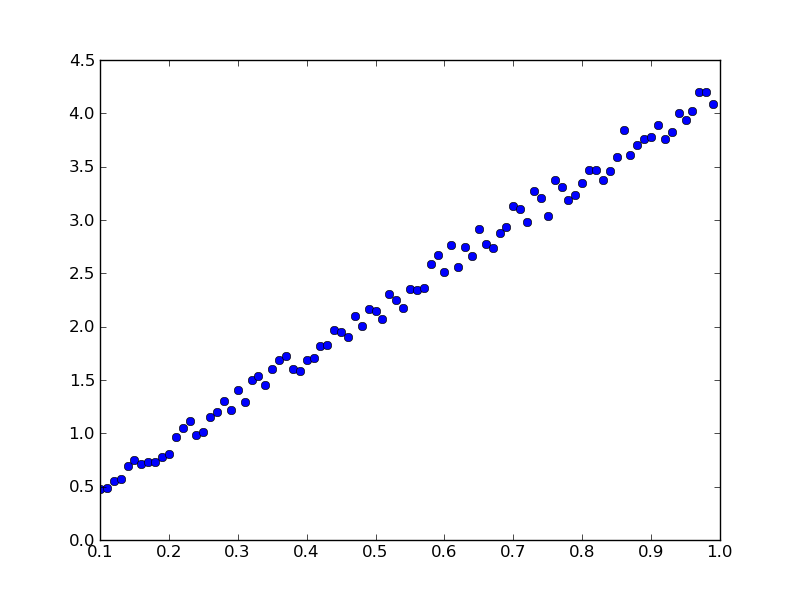
\includegraphics[width=4in]{data/L-Tsq-points}
\end{figure}
\end{frame}

\begin{frame}[fragile]
\frametitle{$L$ vs. $T^2$ - Line}
This line does not make any mathematical sense.
\vspace{-0.1in}
\begin{figure}
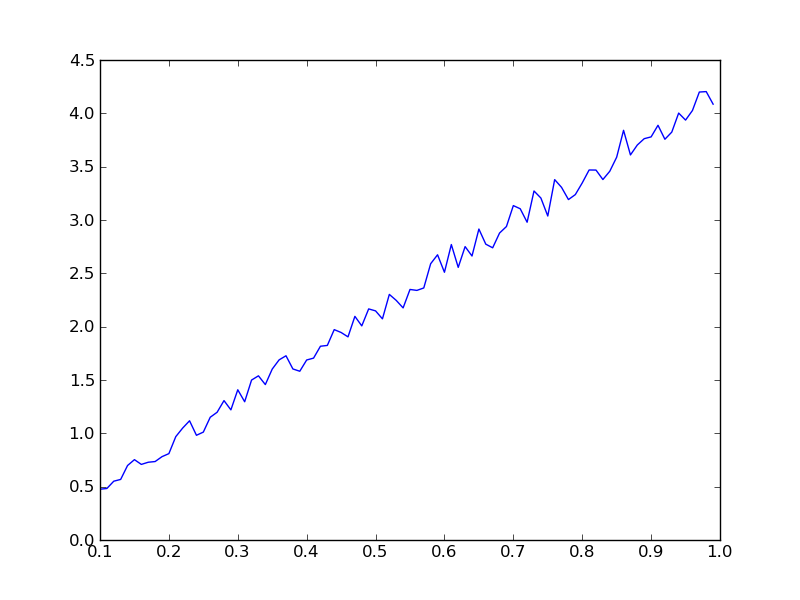
\includegraphics[width=4in]{data/L-Tsq-Line}
\end{figure}
\end{frame}

\begin{frame}[fragile]
\frametitle{$L$ vs. $T^2$ - Least Square Fit}
This is what our intention is.
\vspace{-0.1in}
\begin{figure}
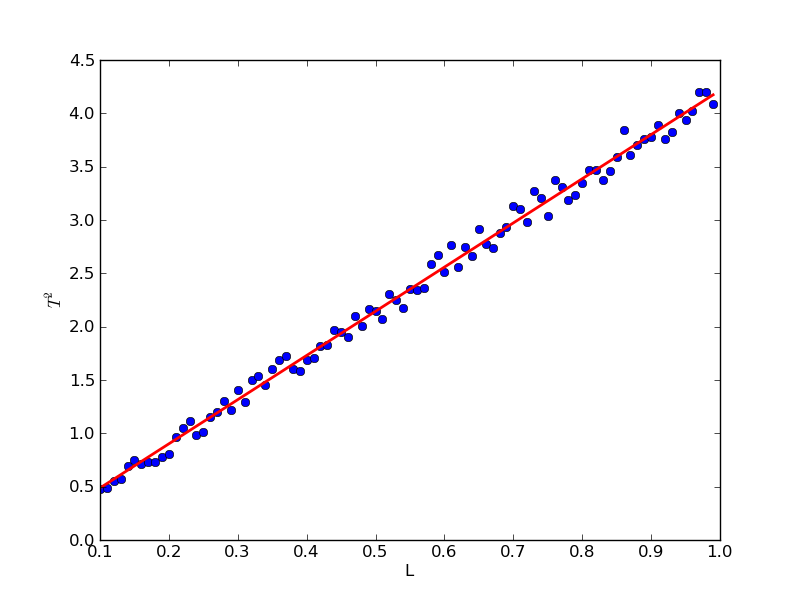
\includegraphics[width=4in]{data/least-sq-fit}
\end{figure}
\end{frame}

\begin{frame}[fragile]
\frametitle{Matrix Formulation}
\begin{itemize}
\item We need to fit a line through points for the equation $T^2 = m \cdot L+c$
\item In matrix form, the equation can be represented as $T_{sq} = A \cdot p$, where $T_{sq}$ is
  $\begin{bmatrix}
  T^2_1 \\
  T^2_2 \\
  \vdots\\
  T^2_N \\
  \end{bmatrix}$
, A is   
  $\begin{bmatrix}
  L_1 & 1 \\
  L_2 & 1 \\
  \vdots & \vdots\\
  L_N & 1 \\
  \end{bmatrix}$
  and p is 
  $\begin{bmatrix}
  m\\
  c\\
  \end{bmatrix}$
\item We need to find $p$ to plot the line
\end{itemize}
\end{frame}

\begin{frame}[fragile]
\frametitle{Getting $L$ and $T^2$}
%If you \alert{closed} IPython after session 2
\begin{lstlisting}
In []: L = []
In []: t = []
In []: for line in open('pendulum.txt'):
  ....     point = line.split()
  ....     L.append(float(point[0]))
  ....     t.append(float(point[1]))
  ....
  ....
\end{lstlisting}
\end{frame}

\begin{frame}[fragile]
\frametitle{Getting $L$ and $T^2$ \dots}
\begin{lstlisting}
In []: L = array(L)
In []: t = array(t)
\end{lstlisting}
\alert{\typ{In []: tsq = t*t}}
\end{frame}
 
\begin{frame}[fragile]
\frametitle{Generating $A$}
\begin{lstlisting}
In []: A = array([L, ones_like(L)])
In []: A = A.T
\end{lstlisting}
%% \begin{itemize}
%% \item A is also called a Van der Monde matrix
%% \item It can also be generated using \typ{vander}
%% \end{itemize}
%% \begin{lstlisting}
%% In []: A = vander(L, 2)
%% \end{lstlisting}
\end{frame}

\begin{frame}[fragile]
\frametitle{\typ{lstsq} \ldots}
\begin{itemize}
\item Now use the \typ{lstsq} function
\item Along with a lot of things, it returns the least squares solution
\end{itemize}
\begin{lstlisting}
In []: result = lstsq(A,tsq)
In []: coef = result[0]
\end{lstlisting}
\end{frame}

\begin{frame}[fragile]
\frametitle{Least Square Fit Line \ldots}
We get the points of the line from \typ{coef}
\begin{lstlisting}
In []: Tline = coef[0]*L + coef[1]

In []: Tline.shape
\end{lstlisting}
\begin{itemize}
\item Now plot \typ{Tline} vs. \typ{L}, to get the Least squares fit line. 
\end{itemize}
\begin{lstlisting}
In []: plot(L, Tline)
\end{lstlisting}
\end{frame}

\begin{frame}[fragile]
\frametitle{Least Squares Fit}
\vspace{-0.15in}
\begin{figure}
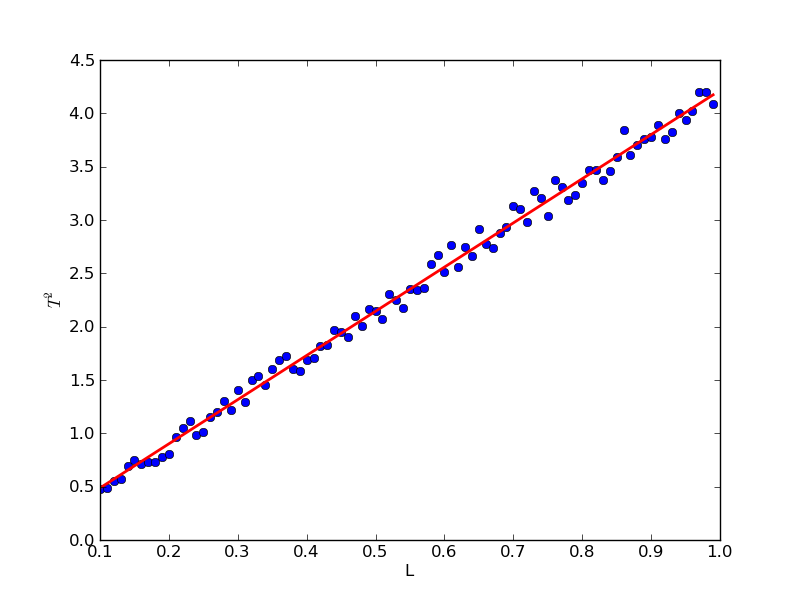
\includegraphics[width=4in]{data/least-sq-fit}
\end{figure}
\end{frame}

\section{Summary}
\begin{frame}
  \frametitle{What did we learn?}
  \begin{itemize}
  \item Matrices
    \begin{itemize}
      \item Initializing
      \item Accessing elements
      \item Slicing and Striding
      \item Transpose
      \item Addition
      \item Multiplication
      \item Inverse of a matrix
      \item Determinant
      \item Eigenvalues and Eigen vector
      %% \item Norms
      %% \item Singular Value Decomposition
    \end{itemize}
  \item Least Square Curve fitting
  \end{itemize}
\end{frame}

\end{document}

%% Questions for Quiz %%
%% ------------------ %%

\begin{frame}[fragile]
\frametitle{\incqno }
\begin{lstlisting}
In []: a = array([[1, 2],
                  [3, 4]])
In []: a[1,0] = 0
\end{lstlisting}
What is the resulting array?
\end{frame}

\begin{frame}[fragile]
\frametitle{\incqno }
\begin{lstlisting}
  In []: x = array(([1,2,3,4],
                    [2,3,4,5]))
  In []: x[-2][-3] = 4
  In []: print x
\end{lstlisting}
What will be printed?
\end{frame}

%% \begin{frame}[fragile]
%% \frametitle{\incqno }
%% \begin{lstlisting}
%%   In []: x = array([[1,2,3,4],
%%                     [3,4,2,5]])
%% \end{lstlisting}
%% What is the \lstinline+shape+ of this array?
%% \end{frame}

\begin{frame}[fragile]
\frametitle{\incqno }
\begin{lstlisting}
  In []: x = array([[1,2,3,4]])
\end{lstlisting}
How to change \lstinline+x+ to \lstinline+array([[1,2,0,4]])+?
\end{frame}

\begin{frame}[fragile]
\frametitle{\incqno }
\begin{lstlisting}
  In []: x = array([[1,2,3,4],
                    [3,4,2,5]])
\end{lstlisting}
How do you get the following slice of \lstinline+x+?
\begin{lstlisting}
array([[2,3],
       [4,2]])
\end{lstlisting}
\end{frame}

\begin{frame}[fragile]
\frametitle{\incqno }
\begin{lstlisting}
  In []: x = array([[9,18,27],
                    [30,60,90],
                    [14,7,1]])
\end{lstlisting}
What is the output of \lstinline+x[::3,::3]+
\end{frame}


\begin{frame}[fragile]
\frametitle{\incqno }
\begin{lstlisting}
In []: a = array([[1, 2],
                  [3, 4]])
\end{lstlisting}
How do you get the transpose of this array?
\end{frame}

\begin{frame}[fragile]
\frametitle{\incqno }
\begin{lstlisting}
In []: a = array([[1, 2],
                  [3, 4]])
In []: b = array([[1, 1],
                  [2, 2]])
In []: a*b
\end{lstlisting}
What does this produce?
\end{frame}

\begin{frame}
\frametitle{\incqno }
What command do you use to find the inverse of a matrix and its
eigenvalues?
\end{frame}

%% \begin{frame}
%% \frametitle{\incqno }
%% The file \lstinline+datafile.txt+ contains 3 columns of data.  What
%% command will you use to read the entire data file into an array?
%% \end{frame}

%% \begin{frame}
%% \frametitle{\incqno }
%% If the contents of the file \lstinline+datafile.txt+ is read into an
%% $N\times3$ array called \lstinline+data+, how would you obtain the third
%% column of this data?
%% \end{frame}

